\documentclass[conference,a4paper]{IEEEtran}

\usepackage[utf8]{inputenc}
\usepackage[T1]{fontenc}
\usepackage[spanish]{babel}
\usepackage{cite}
\usepackage{amsmath}
\usepackage{booktabs}
\usepackage{array}
\usepackage{graphicx}
\usepackage{tikz}
\usepackage{url}
\usepackage{xcolor}
\usepackage{balance}
\usepackage{xspace}
\usepackage[hidelinks]{hyperref}

\hypersetup{
    pdftitle={ArGos: Una Plataforma EASM Orientada a Evidencia y de Alcance Restringido con Integración Multi-Proveedor LLM y MCP},
    pdfauthor={Ruben Torres},
    pdfkeywords={gestión de superficie de ataque, verificación de vulnerabilidades, automatización de ciberseguridad, grandes modelos de lenguaje, Model Context Protocol}
}

\usetikzlibrary{arrows.meta,positioning,fit,shapes.geometric}
\newcommand{\argos}{ArGos\xspace}
\newcommand{\code}[1]{\texttt{#1}}

\title{\argos: Una Plataforma EASM Orientada a Evidencia y de Alcance Restringido\\
con Integración Multi-Proveedor LLM y MCP}

\author{
\IEEEauthorblockN{Rub\'en Torres, \textit{Member, IEEE}}
\IEEEauthorblockA{\textit{Research Department}\\
\textit{STEAM Robotics Academy}\\
San Salvador, El Salvador\\
rtorres.plus25@gmail.com}
\and
\IEEEauthorblockN{Edwin Henriquez}
\IEEEauthorblockA{\textit{Cybersecurity Analyst}\\
\textit{Independent Researcher}\\
San Salvador, El Salvador\\
ehciberseguridad@gmail.com}
\and
\IEEEauthorblockN{Bryan V\'asquez-Pineda, \textit{Member, IEEE}}
\IEEEauthorblockA{\textit{Research Department}\\
\textit{STEAM Robotics Academy}\\
San Salvador, El Salvador\\
cawy.288@gmail.com}
}

\begin{document}

\maketitle

\begin{abstract}
La gestión de la superficie de ataque externa (EASM) une el descubrimiento de activos, la exploración de servicios, la detección de vulnerabilidades, la priorización y la generación de informes, pero su automatización crea dos riesgos prácticos: los escáneres pueden salir del perímetro autorizado y las detecciones no verificadas pueden presentarse como hechos. La asistencia de modelos de lenguaje añade un tercer riesgo porque los banners controlados por atacantes, los nombres de host y los hallazgos pueden convertirse en entradas de inyección indirecta de prompts. Este artículo presenta \argos, una plataforma EASM que trata la autorización, la evidencia y el aislamiento de inquilinos (tenants) como propiedades de primera clase del sistema. Un worker en Go orquesta el descubrimiento de subdominios, la exploración de puertos y HTTP, la inspección TLS, el escaneo basado en firmas, pruebas opcionales de seguridad dinámica de aplicaciones (DAST) y la verificación repetida basada en oráculos. Un Cyber Score determinista expone el desglose de penalizaciones separado de la explicación en lenguaje natural. Las herramientas de datos por inquilino están disponibles tanto para un agente integrado como a través de un servidor HTTP Model Context Protocol (MCP) Streamable. La capa de modelos de lenguaje soporta protocolos nativos de OpenAI, Anthropic y Gemini mientras preserva las llamadas a herramientas, streaming, contabilidad de tokens y metadatos de razonamiento específicos del proveedor. La validación a nivel de artefacto produjo 298 eventos de prueba Go exitosos a través de 30 paquetes y 36 pruebas de frontend exitosas; el análisis estático, la validación con Docker Compose y las pruebas con detector de carreras de datos sobre ocho paquetes críticos de seguridad también se completaron sin fallos. Estos resultados establecen la consistencia de la implementación y el cumplimiento de invariantes clave, no la precisión en la detección de vulnerabilidades. Las brechas empíricas restantes---recall de escaneos a gran escala, reducción de falsos positivos en objetivos en vivo y la evaluación adversarial del límite del LLM---se plantean explícitamente como requisitos de evaluación futura.
\end{abstract}

\begin{IEEEkeywords}
gestión de superficie de ataque, verificación de vulnerabilidades, automatización de ciberseguridad, grandes modelos de lenguaje, Model Context Protocol.
\end{IEEEkeywords}

\section{Introduction}

\begin{figure}[htbp]
\centerline{
\includegraphics[width=0.2\textwidth]{figures/logo.pdf}}
\caption{Logotipo de la plataforma \argos.}
\label{fig:logo}
\end{figure}

La infraestructura expuesta a Internet cambia continuamente a medida que los equipos añaden subdominios, despliegan servicios, rotan certificados y exponen interfaces administrativas. Los sistemas de escaneo rápido como ZMap demostraron que la medición a nivel de Internet puede ser práctica~\cite{Durumeric2013ZMap}; posteriormente Censys demostró cómo el escaneo repetido puede soportar una vista buscable de servicios públicos~\cite{Durumeric2015Censys}. Enterprise EASM reduce esa capacidad a los activos que una organización está autorizada a evaluar y añade priorización, comparación histórica y soporte para la mitigación. El nombre de la plataforma, \argos, está inspirado en Argos Panoptes, el gigante de cien ojos que todo lo ve de la mitología griega, simbolizando el monitoreo continuo y exhaustivo de la superficie de ataque.

El problema de ingeniería no es solo ejecutar escáneres. Primero, el descubrimiento puede producir hosts de terceros o redirecciones, por lo que la autorización debe aplicarse nuevamente en el momento de la ejecución en lugar de asumirse desde una cadena de texto objetivo inicial. Segundo, los hallazgos basados en firmas son observaciones, no vulnerabilidades verificadas automáticamente. Tercero, la severidad por sí sola es una señal de remediación incompleta. Las limitaciones de un único valor del Sistema Común de Puntuación de Vulnerabilidades (CVSS) se han discutido desde los primeros análisis empíricos~\cite{Mell2006CVSS,Scarfone2009CVSS}, mientras que el Sistema de Puntuación de Predicción de Exploits (EPSS) y las encuestas recientes de priorización enfatizan la probabilidad de explotación, el contexto y las múltiples fuentes de evidencia~\cite{Jacobs2021EPSS,Jiang2025Prioritization}. Finalmente, un LLM que lee la salida del escáner está expuesto a texto controlado por el sistema escaneado. La inyección indirecta de prompts puede convertir el contenido recuperado en instrucciones adversariales~\cite{Greshake2023Indirect,Hines2024Spotlighting}.

\argos aborda estas preocupaciones como un sistema integrado en lugar de como envoltorios independientes alrededor de herramientas de seguridad. Su diseño separa el estado de seguridad determinista de la explicación generada, mantiene la identidad del inquilino a través de cada ruta de lectura y coloca puertas de autorización explícitas antes de operaciones activas. La plataforma también expone una superficie de herramientas independiente del modelo a través de MCP, cuyos beneficios de interoperabilidad y riesgos de seguridad son objeto de investigación activa~\cite{Hou2025MCP,Hasan2026MCP}.

Este artículo realiza cuatro contribuciones:
\begin{itemize}
    \item Una tubería EASM de alcance restringido que compone el descubrimiento de activos, la inspección de servicios y TLS, el escaneo de vulnerabilidades, DAST opcional y el enriquecimiento a prueba de fallos, mientras mantiene las etapas centrales fallando de forma segura (fail-closed).
    \item Un modelo de hallazgos orientado a la evidencia que distingue a los candidatos de los hallazgos verificados mediante oráculos repetidos y específicos de su clase, y almacena comprobantes de verificación portables.
    \item Un límite LLM y MCP por inquilino que combina la autorización de herramientas, el seguimiento de ejecución, la contabilidad de tokens y la delimitación explícita del contenido de escaneo no confiable.
    \item Una evaluación a nivel de artefacto de los invariantes implementados, incluyendo pruebas unitarias, de integración, de carreras de datos, de frontend, análisis estático y comprobaciones de configuración de despliegue.
\end{itemize}

La contribución es, por tanto, una arquitectura de sistema y un artefacto de implementación. No es una afirmación de que \argos supera a los escáneres existentes en recall o que su puntuación determinista actual reemplaza a CVSS o EPSS.

\section{Related Work}

\subsection{Discovery and vulnerability scanning}

ZMap introdujo un enfoque sin estado para el escaneo de red de alta velocidad y también discutió prácticas responsables de medición~\cite{Durumeric2013ZMap}. La arquitectura de Censys transformó los escaneos repetidos de protocolos en datos de servicios estructurados y con capacidad de búsqueda~\cite{Durumeric2015Censys}. Estos sistemas motivan el descubrimiento escalable, mientras que \argos se enfoca en la ejecución a nivel de organización, registros longitudinales de escaneos e interpretación orientada al analista. Los escáneres de vulnerabilidades web comúnmente combinan rastreo (crawling), generación de solicitudes y análisis de respuestas~\cite{Chen2020WebScanner}. Trabajos recientes también han explorado añadir IA a clases específicas de vulnerabilidades web~\cite{Manivannan2025AIScanner}; en cambio, \argos mantiene la detección y verificación deterministas y usa el LLM para la selección de herramientas y explicación.

\subsection{Risk prioritization}

CVSS provee un vocabulario de severidad compartido, pero su puntuación no es una estimación directa de explotación en un entorno particular~\cite{Mell2006CVSS,Scarfone2009CVSS}. EPSS introdujo una probabilidad de explotación impulsada por datos y reportó una mejor utilidad de priorización que la práctica basada solo en severidad~\cite{Jacobs2021EPSS}. Una encuesta reciente organiza la priorización de vulnerabilidades por severidad, explotabilidad, contexto y estrategia de agregación~\cite{Jiang2025Prioritization}; el encadenamiento de gestión de vulnerabilidades igualmente combina señales de CVSS, EPSS y vulnerabilidades explotadas conocidas~\cite{Shimizu2025Chaining}. \argos actualmente usa un modelo de penalización transparente y determinista para que la calificación ejecutiva sea reproducible. La incorporación de EPSS, datos de vulnerabilidades explotadas conocidas y la criticidad de activos son trabajo futuro, no una afirmación implementada.

\subsection{LLMs, agents, and MCP in security operations}

ReAct intercala razonamiento y acciones externas, proporcionando un patrón general para agentes de lenguaje que usan herramientas~\cite{Yao2023ReAct}. Las encuestas de operaciones de seguridad asistidas por LLM identifican el triaje de alertas, la gestión de vulnerabilidades, el resumen y la generación de informes como tareas prometedoras, al mismo tiempo que enfatizan las alucinaciones, la privacidad y la robustez adversarial~\cite{Habibzadeh2025LLMSOC,Srinivas2025AISOC}. La inyección de prompts es especialmente relevante cuando la telemetría de seguridad incluye cadenas controladas por el atacante~\cite{Greshake2023Indirect}. Spotlighting propone transformaciones o delimitadores explícitos para el contenido no confiable~\cite{Hines2024Spotlighting}; la investigación sobre barandillas específicas de seguridad argumenta además a favor de controles por capas y un continuo equipo rojo (red-teaming)~\cite{Ali2026SecureCAI}.

MCP estandariza el descubrimiento y la invocación de herramientas accesibles para el modelo. Su interfaz abierta reduce el acoplamiento con los proveedores pero crea riesgos distintos del ciclo de vida y del envenenamiento de herramientas~\cite{Hou2025MCP}. Un estudio empírico de 1,899 servidores MCP de código abierto encontró tanto vulnerabilidades convencionales como debilidades específicas de MCP~\cite{Hasan2026MCP}. Estos hallazgos motivan los esquemas limitados de \argos, la autorización por herramienta, el alcance derivado del inquilino y los registros de auditoría.

\section{System Goals and Threat Model}

\argos asume que un operador inquilino autenticado solo puede escanear dominios verificados o redes de laboratorio permitidas explícitamente. Los hosts descubiertos, destinos de redireccionamiento, contenido HTTP, metadatos de certificados, nombres de plantillas y descripciones de vulnerabilidades no son de confianza. Un token API puede ser robado o tener privilegios excesivos; por lo tanto, la autenticación por sí sola es insuficiente y cada herramienta requiere una decisión de autorización. Los proveedores de LLM son tratados como procesadores externos: la salida del modelo puede ser incorrecta y los protocolos de los proveedores pueden diferir.

El diseño persigue cinco objetivos:
\begin{enumerate}
    \item \textit{Alcance cerrado por fallo (Fail-closed scope)}: los objetivos mal formados, excluidos o no coincidentes se deniegan antes de que se invoque un proceso de escáner.
    \item \textit{Separación de evidencia}: un detector crea un candidato; solo un oráculo exitoso lo promueve a verificado.
    \item \textit{Estado de seguridad determinista}: las puntuaciones y hallazgos brutos no dependen de una respuesta de LLM.
    \item \textit{Acceso derivado del inquilino}: los identificadores del inquilino provienen de la identidad autenticada, nunca de argumentos de herramientas proporcionados por el modelo.
    \item \textit{Portabilidad del proveedor}: el mensaje específico del vendedor, la herramienta, el streaming, el razonamiento y los formatos de uso permanecen detrás de una interfaz.
\end{enumerate}

El modelo de amenazas actual no defiende contra el compromiso del host que ejecuta el worker, binarios maliciosos del escáner o un administrador de bases de datos completamente comprometido. Tampoco prueba que delimitar el texto no confiable derrote todos los ataques de inyección de prompts.

\section{Architecture and Implementation}

La Fig.~\ref{fig:architecture} muestra las rutas de control y datos. El cliente de Vue llama a un plano de control HTTP en Go. Los trabajos de escaneo son ejecutados por un worker separado en Go, permitiendo que la concurrencia del escaneo y la salida de red estén aisladas de la API. PostgreSQL almacena objetivos, escaneos, hallazgos, evidencia, puntuaciones, historial de chat, uso de tokens y registros de auditoría de MCP, todo esto restringido por inquilino. El asistente integrado y el servidor MCP comparten almacenes de dominio y el mismo registro de proveedores de LLM.

\begin{figure*}[t]
\centering
\begin{tikzpicture}[
    font=\footnotesize,
    node distance=7mm and 10mm,
    box/.style={draw=blue!55, rounded corners=2pt, fill=blue!5, align=center,
                minimum width=28mm, minimum height=10mm, inner sep=3pt},
    sec/.style={draw=orange!70, rounded corners=2pt, fill=orange!8, align=center,
                minimum width=29mm, minimum height=10mm, inner sep=3pt},
    data/.style={draw=teal!60, rounded corners=2pt, fill=teal!7, align=center,
                 minimum width=29mm, minimum height=10mm, inner sep=3pt},
    flow/.style={-{Latex[length=2mm]}, line width=0.55pt, draw=gray!70}
]
\node[box] (ui) {Vue client\\analyst UI};
\node[box, right=of ui] (api) {Go API\\control plane};
\node[sec, right=of api] (scope) {Identity, target\\verification, scope};
\node[box, right=of scope] (worker) {Go scan worker\\orchestrator};

\node[data, below=11mm of api] (db) {PostgreSQL\\tenant-scoped state};
\node[sec, below=11mm of scope] (verify) {Oracle verifier\\N/N receipts};
\node[box, below=11mm of worker] (tools) {subfinder, naabu, httpx,\\tlsx, nuclei, katana};

\node[box, below=11mm of ui] (agent) {Integrated agent\\bounded tool loop};
\node[box, below=11mm of db] (mcp) {MCP Streamable HTTP\\typed tools and audit};
\node[data, below=11mm of verify] (llm) {Provider registry\\OpenAI, Anthropic, Gemini};

\draw[flow] (ui) -- (api);
\draw[flow] (api) -- (scope);
\draw[flow] (scope) -- (worker);
\draw[flow] (worker) -- (tools);
\draw[flow] (tools) -- (verify);
\draw[flow] (verify) -- (db);
\draw[flow] (api) -- (db);
\draw[flow] (agent) -- (db);
\draw[flow] (mcp) -- (db);
\draw[flow] (agent) -- (llm);
\draw[flow] (mcp) -- (llm);
\draw[flow] (ui) -- (agent);
\end{tikzpicture}
\caption{Arquitectura de \argos. La autorización precede al escaneo activo; los hallazgos deterministas, la evidencia y las puntuaciones se persisten antes de la explicación opcional del LLM.}
\label{fig:architecture}
\end{figure*}

\subsection{Scope-constrained scan pipeline}

El ejecutor de alcance acepta dominios exactos, comodines (wildcards), CIDRs y una lista separada de permitidos para CIDR de laboratorio. Antes de autorizar un escaneo, el inquilino debe verificar el dominio objetivo para demostrar su propiedad. Esto se logra desplegando un registro DNS TXT específico o alojando un archivo \code{.well-known/argos-verification} en el servidor web. Las exclusiones explícitas de dominio y red tienen prioridad. La resolución DNS está deshabilitada por defecto; si se habilita, todas las direcciones resueltas se comprueban contra exclusiones y redes permitidas. Los adaptadores de ProjectDiscovery repiten la verificación de alcance inmediatamente antes de la ejecución del proceso. Esta segunda comprobación es importante porque la tubería puede recibir hosts del descubrimiento y rastreo en lugar de directamente del usuario.

El worker ejecuta las siguientes etapas:
\begin{equation}
\begin{split}
\mathrm{target} &\rightarrow \mathrm{subdomains} \rightarrow \mathrm{ports} \\
&\rightarrow \mathrm{HTTP} \rightarrow \mathrm{TLS} \rightarrow \mathrm{nuclei} \\
&\rightarrow [\mathrm{crawl} \rightarrow \mathrm{DAST}] \rightarrow [\mathrm{verify}].
\end{split}
\label{eq:pipeline}
\end{equation}
La enumeración de subdominios, el sondeo HTTP y el escaneo de firmas son etapas centrales. La inspección de puertos y TLS, DAST, y la verificación de oráculos son etapas de enriquecimiento: se registra un fallo local y el escaneo puede continuar a menos que se cancele el contexto. DAST es opcional (opt-in) porque inyecta payloads. Los límites de host, perfiles de tasa de peticiones, tiempos de espera y la cancelación proporcionan barreras de recursos.

\subsection{Evidence-oriented verification}

Cada hallazgo recibe una huella (fingerprint) estable derivada de campos de identificación normalizados. El verificador mapea las señales de la plantilla admitidas a una de las 26 clases de oráculos, que incluyen paneles expuestos, listado de directorios, CORS, métodos HTTP inseguros, XSS reflejado o almacenado, variantes de inyección SQL, SSRF, XXE, JWT \code{alg:none}, IDOR, desincronización HTTP, confusión de tipos y asignación masiva. Las clases de oráculo intrusivo requieren tanto la habilitación de DAST como un objetivo dentro del alcance.

Un oráculo repite un chequeo idempotente $N$ veces, donde $N=2$, $3$ o $5$ para perfiles sigiloso (stealth), normal o agresivo. Un candidato solo es promovido cuando
\begin{equation}
    \mathrm{verified}(f) \iff \mathrm{successes}(f)=\mathrm{attempts}(f)>0.
\end{equation}
Los errores técnicos no refutan un hallazgo; lo dejan como candidato. Una verificación exitosa almacena la receta redactada, evidencia de petición/respuesta, recuento de intentos, tipo de oráculo y la huella. Este comprobante admite futuras auditorías y re-verificaciones sin necesidad de pedir a un LLM que juzgue la explotabilidad.

\subsection{Transparent scoring}

El Cyber Score convierte el escaneo actual en un número y letra mientras preserva su desglose. Sea $F$ los hallazgos y $C$ los certificados observados. La implementación actual calcula
\begin{equation}
S=\max\left(0,100-\sum_{f\in F}w(s_f)-\sum_{c\in C}t(c)\right),
\end{equation}
donde $w$ asigna penalizaciones de 40, 20, 8, 3 y 1 a hallazgos críticos, altos, medios, bajos e informacionales. La función TLS asigna 15 a un certificado expirado y 10 a un certificado autofirmado o versión obsoleta de SSL/TLS. Las calificaciones A--F corresponden a los umbrales 90, 80, 70, 60 y 50. Este modelo es intencionalmente simple y explicable; la interfaz muestra tanto $S$ como los componentes de la penalización. No debe interpretarse como una probabilidad de explotación.

\subsection{Tenant-aware agent and MCP surface}

El asistente usa un ciclo de herramientas acotado con un máximo de cinco iteraciones LLM. Las herramientas enumeran dominios y escaneos, recuperan resúmenes, filtran hallazgos e inspeccionan problemas de puertos y TLS. Los resultados se insertan en el contexto del modelo con un marcador explícito que indica que los datos del escaneo no son de confianza y no deben tratarse como instrucciones. Esta es una defensa de marcado de datos inspirada en spotlighting~\cite{Hines2024Spotlighting}, pero el sistema no afirma tener resistencia formal frente a ataques adaptativos.

El servidor MCP expone los mismos conceptos por inquilino a través de herramientas fuertemente tipadas. Las claves API tipo portador (bearer) se almacenan como hashes y se resuelven en una identidad que contiene inquilino, token y alcances. El middleware de autorización se ejecuta por cada llamada a herramienta; el rastreo de ejecución almacena un hash de los argumentos, resultado, latencia y tamaño del resultado. Anotaciones de solo lectura se aplican a herramientas de datos, mientras que el escalado experto está marcado explícitamente como que cambia el estado. Los escaneos entre inquilinos no devuelven datos, incluso si un modelo suministra un identificador de escaneo diferente.

\subsection{Native multi-provider LLM layer}

Una interfaz de proveedor cubre el chat síncrono, streaming, definiciones de herramientas, llamadas a herramientas y el uso de tokens. Una fábrica a prueba de hilos (thread-safe) reemplaza atómicamente el conjunto de proveedores activo cuando cambian las opciones ambientales alternativas o la configuración cifrada de la base de datos. Los endpoints compatibles con OpenAI utilizan el contrato de finalización de chat. Anthropic y Gemini usan su mensaje nativo, herramienta, streaming, uso y estructuras de razonamiento; los identificadores del catálogo se traducen a identificadores de modelos API exactos. Los metadatos del proveedor retienen las firmas de razonamiento de Anthropic y las firmas de pensamiento de Gemini a través de viajes de ida y vuelta de las herramientas. La interfaz registra el uso de tokens de prompt y completion sin hacer que el texto generado forme parte del Cyber Score.

\section{Operational Interface}

La interfaz presenta el estado determinista del escaneo antes de la interpretación generada. La Fig.~\ref{fig:ui-analysis} muestra un registro de escaneo y una respuesta del asistente sobre los mismos datos operativos. Las capturas de pantalla son artefactos de demostración, no resultados de experimentos cuantitativos.

\begin{figure*}[t]
    \centering
    \begin{minipage}[t]{0.49\textwidth}
        \centering
        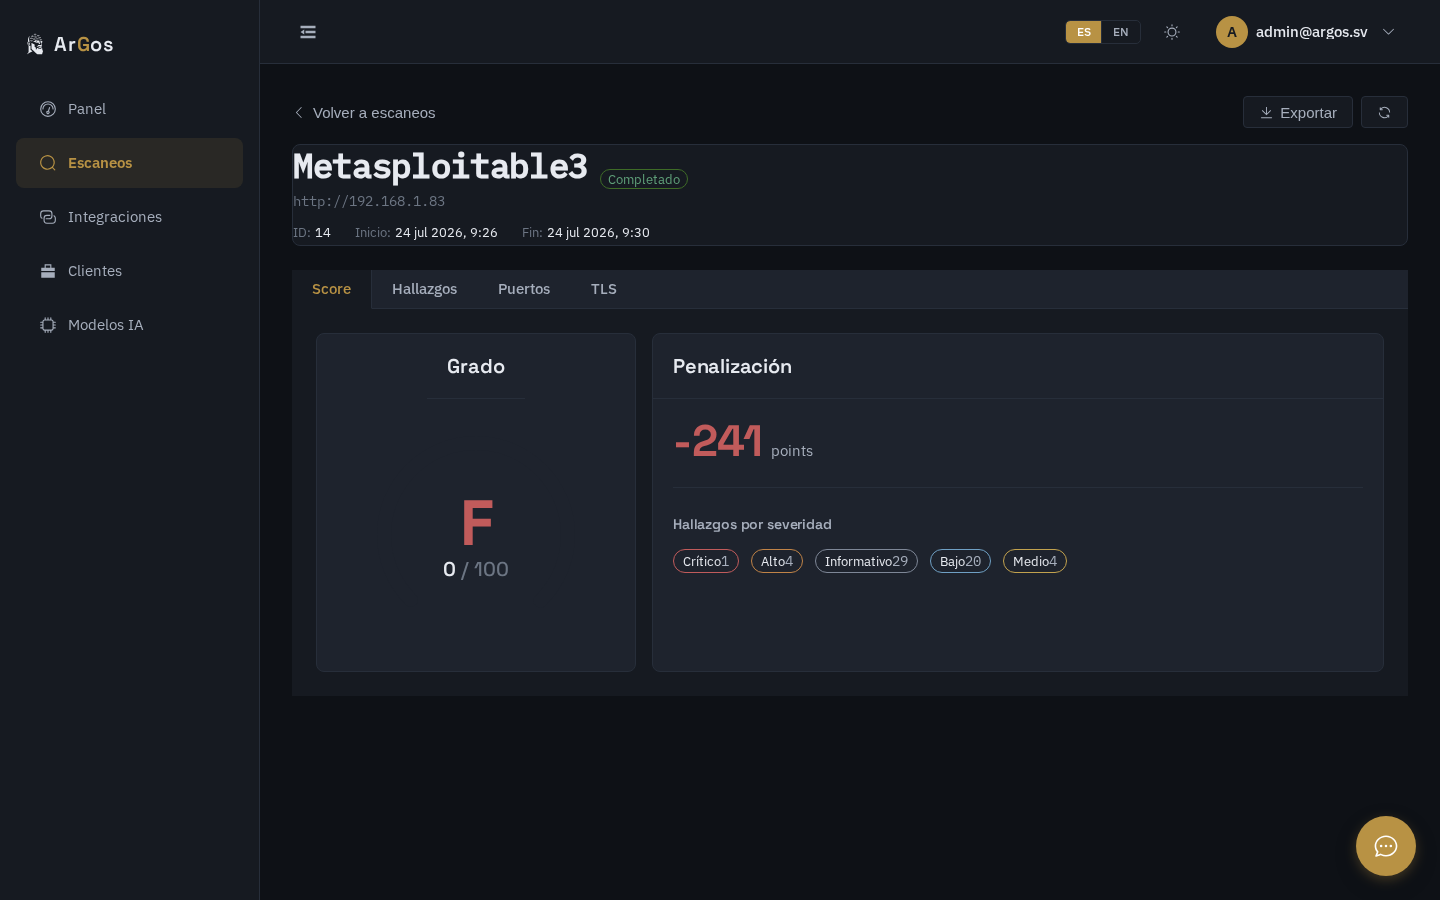
\includegraphics[width=\linewidth]{figures/scan-detail.png}
        \small (a) Detalle del escaneo con calificación y desglose de penalizaciones.
    \end{minipage}
    \hfill
    \begin{minipage}[t]{0.49\textwidth}
        \centering
        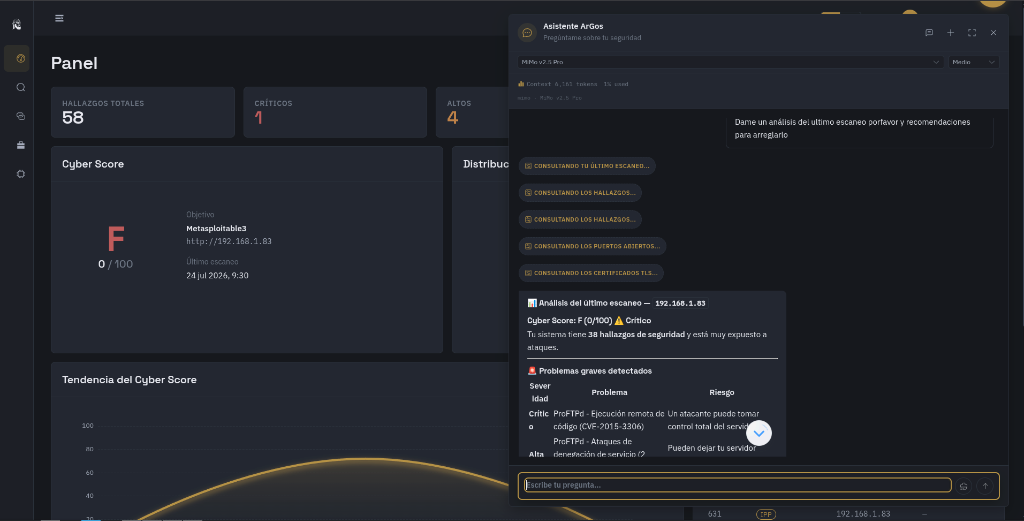
\includegraphics[width=\linewidth]{figures/chatbot-response.png}
        \small (b) Explicación asistida por herramientas mostrada junto al contexto de escaneo.
    \end{minipage}
    \caption{Flujo de trabajo del analista en la demostración de \argos. La explicación generada aumenta, pero no reemplaza, los hallazgos persistidos y los componentes de la puntuación.}
    \label{fig:ui-analysis}
\end{figure*}

La Fig.~\ref{fig:ui-governance} ilustra dos límites de gobernanza: la configuración del proveedor es una función administrativa, y un panel de control para el inquilino expone solo el estado a nivel de la organización. La interfaz de usuario puede cambiar el idioma y el tema, pero estas opciones de presentación no alteran la autorización.

\begin{figure*}[t]
    \centering
    \begin{minipage}[t]{0.49\textwidth}
        \centering
        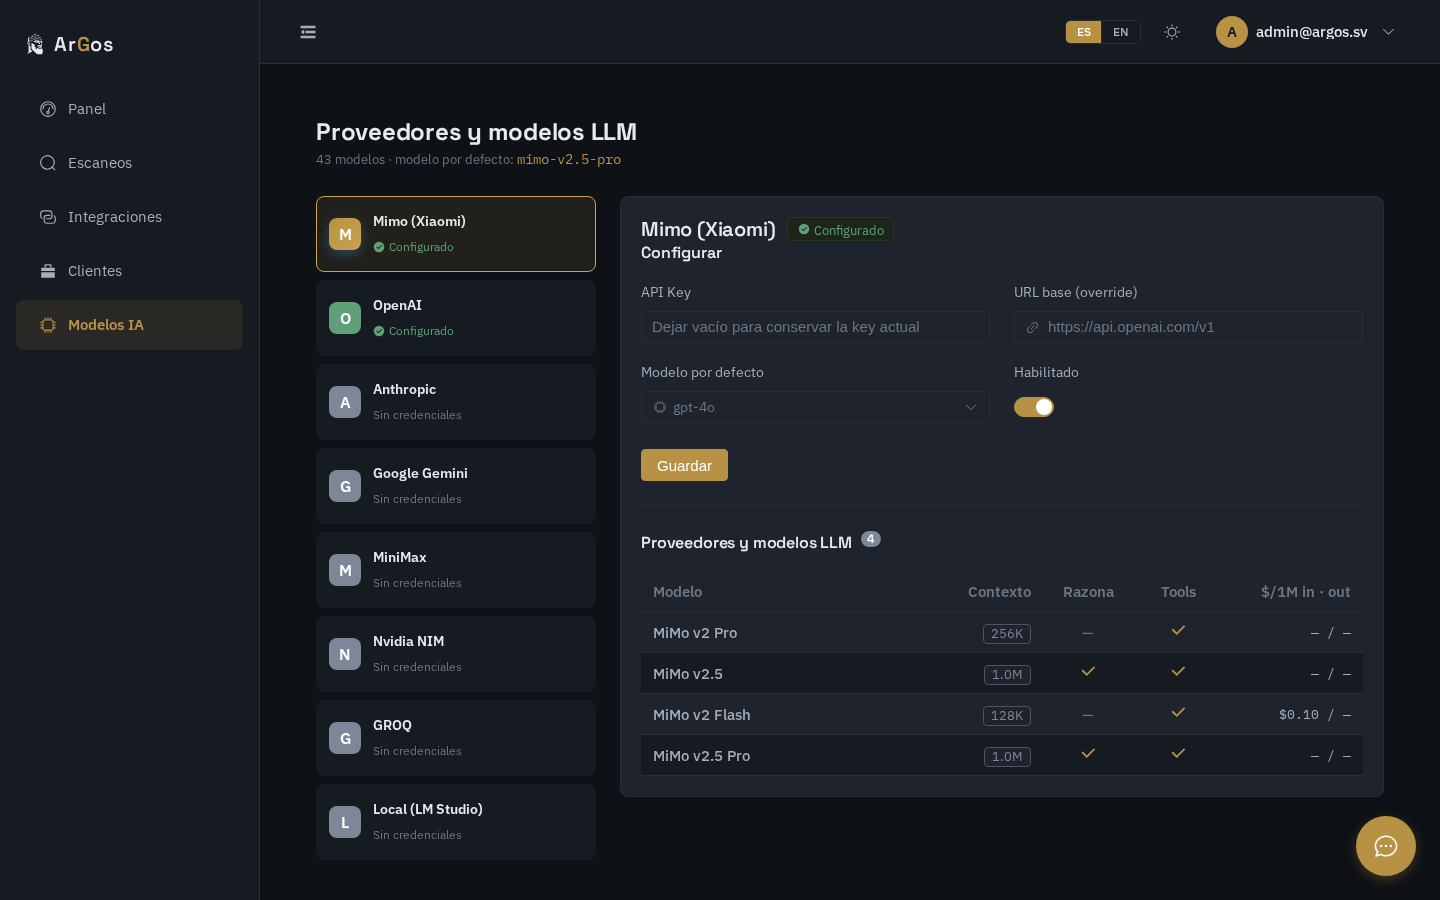
\includegraphics[width=\linewidth]{figures/ai-providers.png}
        \small (a) Configuración administrativa del proveedor y modelos.
    \end{minipage}
    \hfill
    \begin{minipage}[t]{0.49\textwidth}
        \centering
        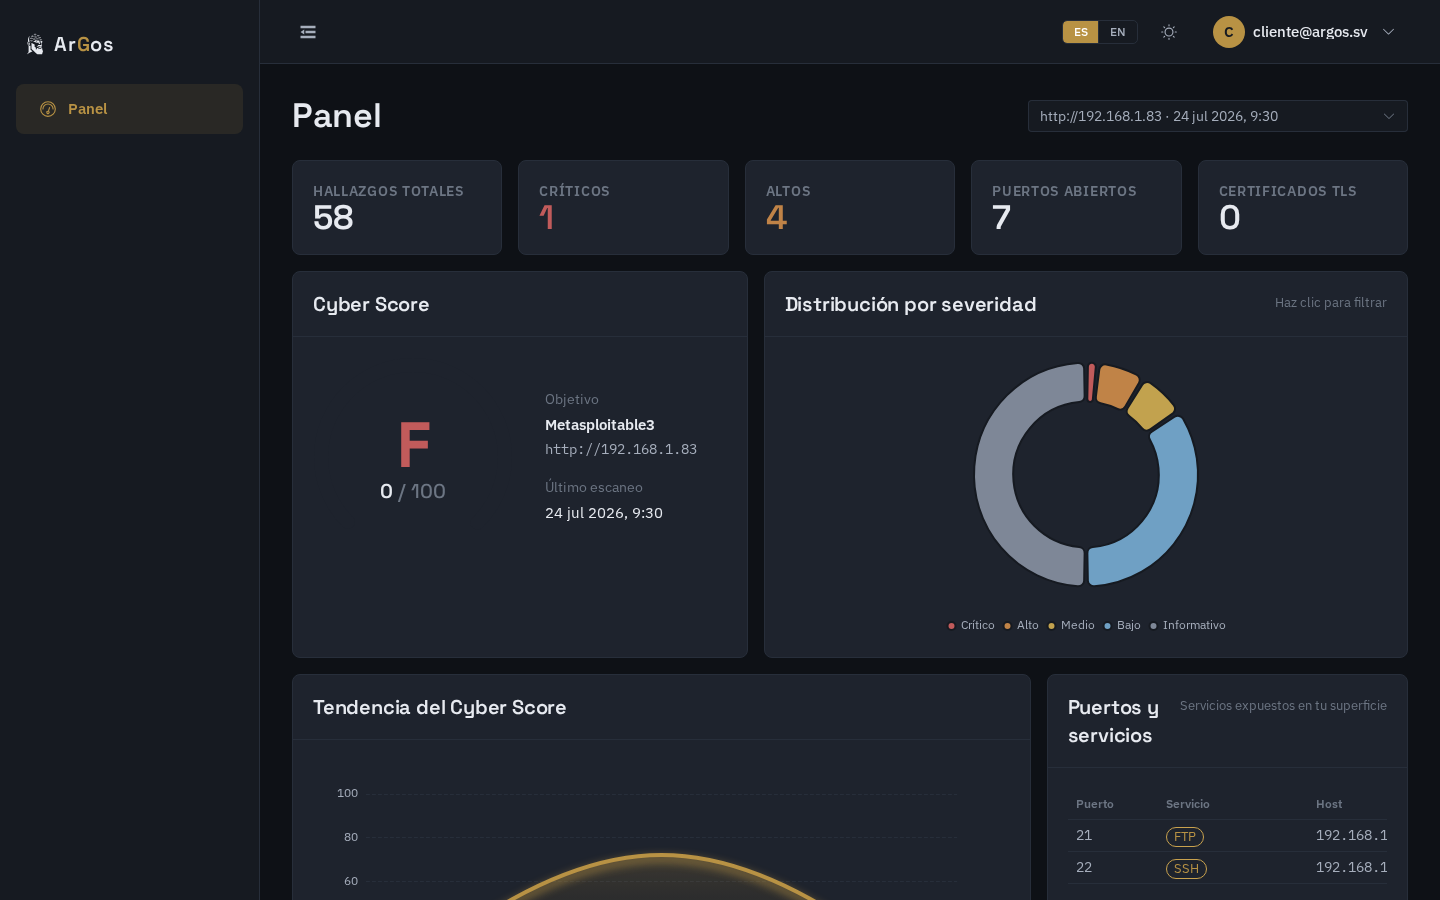
\includegraphics[width=\linewidth]{figures/tenant-dashboard.png}
        \small (b) Tablero de postura restringido por inquilino.
    \end{minipage}
    \caption{Gobernanza del proveedor y aislamiento del inquilino en la interfaz web. Las credenciales de la API no se devuelven al frontend después de su persistencia.}
    \label{fig:ui-governance}
\end{figure*}

\section{Evaluation}

\subsection{Research questions}

La evaluación formula cuatro preguntas de investigación a nivel de artefacto: \textbf{RQ1}: ¿rechazan los límites de alcance y de inquilino las entradas no autorizadas? \textbf{RQ2}: ¿preservan los componentes de oráculo y evidencia la distinción entre candidato y verificado? \textbf{RQ3}: ¿los adaptadores MCP y de proveedor preservan la autorización, la semántica del protocolo nativo, el streaming, las herramientas y el uso? \textbf{RQ4}: ¿aprueba el repositorio completo sus puertas de calidad automatizadas?

\subsection{Environment and procedure}

La evaluación usó Linux 7.1.5 en x86-64, Go 1.26.5, Node.js 26.4.0, pnpm 11.9.0 y Vitest 4.1.9. El árbol de trabajo evaluado se basó en el commit \code{71f8bd4}. Las pruebas de backend se ejecutaron con \code{go test -json ./\ldots}; el número reportado es la cuenta de eventos de pruebas Go exitosas, incluyendo sub-pruebas con nombre, en lugar de una afirmación de 298 propiedades de seguridad independientes. Los paquetes críticos de seguridad se volvieron a ejecutar luego con el detector de carreras (race detector) de Go. La suite frontend se ejecutó una vez en modo no-watch. El análisis estático y la sintaxis de despliegue se verificaron con \code{go vet ./\ldots} y \code{docker compose config --quiet}.

\begin{table}[t]
\centering
\caption{Resumen de validación automatizada}
\label{tab:validation}
\begin{tabular}{p{0.32\columnwidth}p{0.43\columnwidth}r}
\toprule
Capa & Foco de validación & Exitosas \\
\midrule
Oráculo & Verificaciones diferenciales y evidencia & 62 \\
API HTTP & Autenticación, manejadores, actualización de proveedores & 22 \\
Adaptadores LLM & Peticiones nativas, flujos, herramientas, uso & 22 \\
Alcance & Dominio, CIDR, exclusión, comportamiento DNS & 21 \\
Escaneo & Tubería, cancelación, desduplicación & 20 \\
Evidencia & Captura, hash, integridad & 12 \\
MCP & Autenticación, delimitación, paginación, transporte HTTP & 12 \\
Otros paquetes Go & Comportamiento del dominio y adaptador & 127 \\
Frontend Vue & Componentes y cliente API & 36 \\
\midrule
Total & Eventos de prueba Go más pruebas de frontend & 334 \\
\bottomrule
\end{tabular}
\end{table}

Los 298 eventos de pruebas de Go fueron exitosos a través de 30 paquetes con cero eventos fallidos. Todas las 36 pruebas de frontend en seis archivos pasaron. La Tabla~\ref{tab:validation} desglosa los paquetes más relevantes para el artículo; el resto de los paquetes Go incluyen recuperación de conocimiento, claves API, gobernanza, orquestación, exportaciones y adaptadores de ejecución.

\begin{table}[t]
\centering
\caption{Comprobaciones orientadas a invariantes}
\label{tab:invariants}
\begin{tabular}{p{0.29\columnwidth}p{0.57\columnwidth}}
\toprule
Invariante & Comprobación automatizada representativa \\
\midrule
Confinamiento de alcance & Coincidencia exacta/comodín/CIDR, precedencia de exclusión, objetivos mal formados y no resueltos, adaptadores de escáner en alcance. \\
Aislamiento de inquilinos & Rechazado el resumen de MCP entre inquilinos; las listas de dominios de inquilinos no pueden exponer a otro inquilino. \\
Límite de evidencia & Los candidatos fuera de alcance y no repetibles no se promueven; los hallazgos verificados retienen los recibos. \\
Puerta DAST & Clases de oráculos intrusivos requieren habilitación explícita de DAST. \\
Autenticación MCP & Llave portadora faltante rechazada; la llave generada lista herramientas sobre Streamable HTTP. \\
Semántica de proveedor & Llamadas de herramientas nativas de Anthropic/Gemini, uso de streaming, firmas de razonamiento y despacho de modelos comprobados contra contratos HTTP falsos (mocks). \\
\bottomrule
\end{tabular}
\end{table}

Las pruebas con detector de carreras de datos pasaron para los paquetes de alcance, puntuación, escaneo, verificador, oráculo, MCP, LLM y asistente. \code{go vet} no reportó fallos, y la validación de la configuración de Docker Compose tuvo éxito. Estos resultados responden las preguntas RQ1--RQ4 al nivel de implementación: los invariantes probados se mantienen para los casos codificados y los contratos de protocolo falsos (mock).

\subsection{What the evaluation does not establish}

La validación no compara a \argos con productos EASM comerciales, no estima el recall de descubrimiento, ni mide la reducción de falsos positivos en un corpus representativo en vivo. No hace llamadas API de pago reales a OpenAI, Anthropic o Gemini; las pruebas de proveedor utilizan servidores HTTP controlados que aseguran las formas documentadas de peticiones nativas y streaming. Tampoco evalúa si un modelo de lenguaje responde correctamente a los conjuntos de tareas MCP o si resiste la inyección adaptativa de prompts. Estas distinciones evitan que se reporte erróneamente el pase de pruebas de software como eficacia de seguridad.

\section{Discussion}

La arquitectura demuestra una separación útil de responsabilidades. Los componentes deterministas deciden el alcance, recolectan evidencia y calculan la puntuación; el LLM selecciona las herramientas de lectura y convierte el estado persistido en lenguaje. Esto reduce la consecuencia de una alucinación porque una explicación generada no puede mutar silenciosamente el grado subyacente o el veredicto de verificación. Los adaptadores nativos del proveedor también evitan forzar APIs de vendedores a través de una aproximación compatible con OpenAI, lo cual es importante para las firmas de llamadas de herramientas y la contabilidad de tokens.

La regla N/N del verificador favorece la precisión y la auditabilidad sobre la promoción agresiva. Su principal debilidad es la cobertura: los hallazgos no compatibles siguen siendo candidatos, y un oráculo determinista aún puede codificar una condición incompleta. Los recibos (receipts) hacen que esta limitación sea inspeccionable, pero no la eliminan. De igual forma, el Cyber Score es transparente pero actualmente omite la probabilidad de explotación, la criticidad de los activos, la duración de la exposición y los controles compensatorios. La literatura de priorización sugiere que estas señales deberían agregarse como factores separados y atribuibles en lugar de ocultarse dentro de la prosa generada~\cite{Jacobs2021EPSS,Jiang2025Prioritization,Shimizu2025Chaining}.

MCP crea un límite de herramientas explícito, pero las descripciones de herramientas, esquemas, dependencias y contenido devuelto siguen siendo superficies de ataque~\cite{Hou2025MCP,Hasan2026MCP}. \argos mitiga algunos de estos riesgos a través de conjuntos de herramientas limitados, identidad derivada del alcance, auditoría y marcado de datos no confiables. Evaluaciones futuras de tipo equipo rojo (red-team) deben incluir nombres de hosts maliciosos, descripciones de vulnerabilidades, evidencia de escaneo almacenada, manipulación de argumentos de llamadas de herramientas y respuestas de proveedores comprometidos.

\section{Limitations and Threats to Validity}

\textit{Validez de constructo}: pasar las pruebas mide la conformidad con el comportamiento codificado, no la precisión de la detección de vulnerabilidades o la reducción del riesgo operativo. La salida de puntuación A--F es una abstracción de gestión interna más que una métrica estandarizada.

\textit{Validez interna}: los servidores HTTP falsos (mocks) aíslan los contratos de los proveedores pero no pueden capturar todos los cambios en las APIs de producción, límites de velocidad o comportamientos de red. Los recuentos de eventos de prueba incluyen sub-pruebas y se informan como tales. Las capturas de pantalla contienen datos de demostración y no se tratan como mediciones experimentales.

\textit{Validez externa}: el artefacto aún no ha sido evaluado frente a diversos dominios empresariales, proveedores en la nube, condiciones de red o versiones de escáneres. Los objetivos de laboratorio como OWASP Juice Shop, DVWA y Metasploitable3 son intencionalmente vulnerables y no representan la prevalencia de producción.

\textit{Validez de seguridad}: los chequeos de alcance y puertas DAST reducen el sobrealcance accidental pero no reemplazan la autorización legal o el control de cambios operativo. El datamarking es solo una capa contra la inyección de prompts, y no se afirma que sea una defensa universal.

\section{Conclusion and Future Work}

Este artículo presentó \argos, una plataforma EASM de alcance restringido y orientada a la evidencia, que integra el escaneo determinista y la puntuación con LLM de inquilino y las interfaces MCP. La implementación obliga a que exista autorización antes de la ejecución activa, separa los hallazgos candidatos de los verificados a través de oráculos repetidos, y mantiene la explicación generada fuera de la fuente de la verdad. Los adaptadores nativos para OpenAI, Anthropic y Gemini preservan la semántica de uso y herramientas específicas de los vendedores detrás de una interfaz de proveedor. La validación automatizada fue superada en todo momento, abarcando las pruebas de backend, frontend, de carreras, análisis estático y comprobaciones de la configuración de despliegue.

La próxima fase de evaluación debería ejecutar escaneos longitudinales controlados sobre objetivos propios e informar el recall de descubrimiento de activos, la precisión de los hallazgos, el rendimiento de verificación, el tiempo de ejecución y el volumen de peticiones por perfil de intensidad. La priorización debería incorporar EPSS, señales de vulnerabilidad explotada conocida, criticidad de activos y exposición temporal como factores visibles separadamente. La capa MCP debe ser evaluada con conjuntos de preguntas multi-herramienta estables y corpus de inyección de prompt adversarios. Finalmente, las pruebas de conformidad con proveedores en vivo deberían complementar los contratos mock mientras se redactan los datos del inquilino y se controla el costo.

\section*{Artifact Availability}

El repositorio contiene el backend de Go, el frontend de Vue, el contrato de OpenAPI, las migraciones de bases de datos, el laboratorio Docker Compose, las pruebas, las capturas de pantalla y el código fuente LaTeX de este documento. Los PDF de la investigación revisada se retienen localmente como material de investigación y se excluyen de las versiones del producto.

\section*{Acknowledgment}

El autor agradece a los mantenedores de las herramientas de escaneo de ProjectDiscovery y a los investigadores cuyos documentos, disponibles abiertamente, informaron el diseño y el análisis de limitaciones.

\balance
\bibliographystyle{IEEEtran}
\bibliography{references}

\end{document}
